\documentclass[11pt]{amsart}
\usepackage[margin=1in]{geometry}
\usepackage{amsmath,amssymb,amsthm,mathtools}
\usepackage{graphicx}
\usepackage{hyperref}

\newtheorem{theorem}{Theorem}
\newtheorem{lemma}{Lemma}
\newtheorem{proposition}{Proposition}
\newtheorem{corollary}{Corollary}
\theoremstyle{remark}
\newtheorem{remark}{Remark}

\newcommand{\Z}{\mathbb Z}
\newcommand{\N}{\mathbb N}
\newcommand{\ellp}{\ell_p(\Z)}
\newcommand{\cz}{c_0(\Z)}
\newcommand{\norm}[1]{\left\|#1\right\|}
\newcommand{\abs}[1]{\left|#1\right|}
\newcommand{\Per}{\operatorname{Per}}
\newcommand{\PSP}{\operatorname{PSP}}

\title[Periodic Shadowing on \(\ell_p\) and \(c_0\)]{Periodic Shadowing for Bilateral Weighted Shifts is the Same on \(\ell_p(\mathbb Z)\) and \(c_0(\mathbb Z)\)}
\author{Agent lane 17}
\date{2026-07-18}

\begin{document}

\begin{abstract}
We answer Question 4.13 of Hevessy--Raunig's paper \emph{Dynamical properties of weighted shifts on sequence spaces}.  Let \(w=(w_n)_{n\in\Z}\) be bounded and bounded away from zero, and let \(B_w\) be the bilateral weighted backward shift.  Then, for every \(1\leq p<\infty\), \(B_w\) has the periodic shadowing property on \(\ell_p(\Z)\) if and only if it has the periodic shadowing property on \(c_0(\Z)\).  The same answer holds for bilateral weighted forward shifts.
\end{abstract}

\maketitle

\section{Source Question}

The source paper studies the bilateral weighted backward shift
\[
 B_w(x)_j=w_{j+1}x_{j+1}
\]
on \(\ell_p(\Z)\), \(1\leq p<\infty\), and on \(c_0(\Z)\), where \(w\) is bounded and \(\inf_j |w_j|>0\).  After proving a complete \(c_0\)-characterization of the periodic shadowing property, the authors ask:

\begin{center}
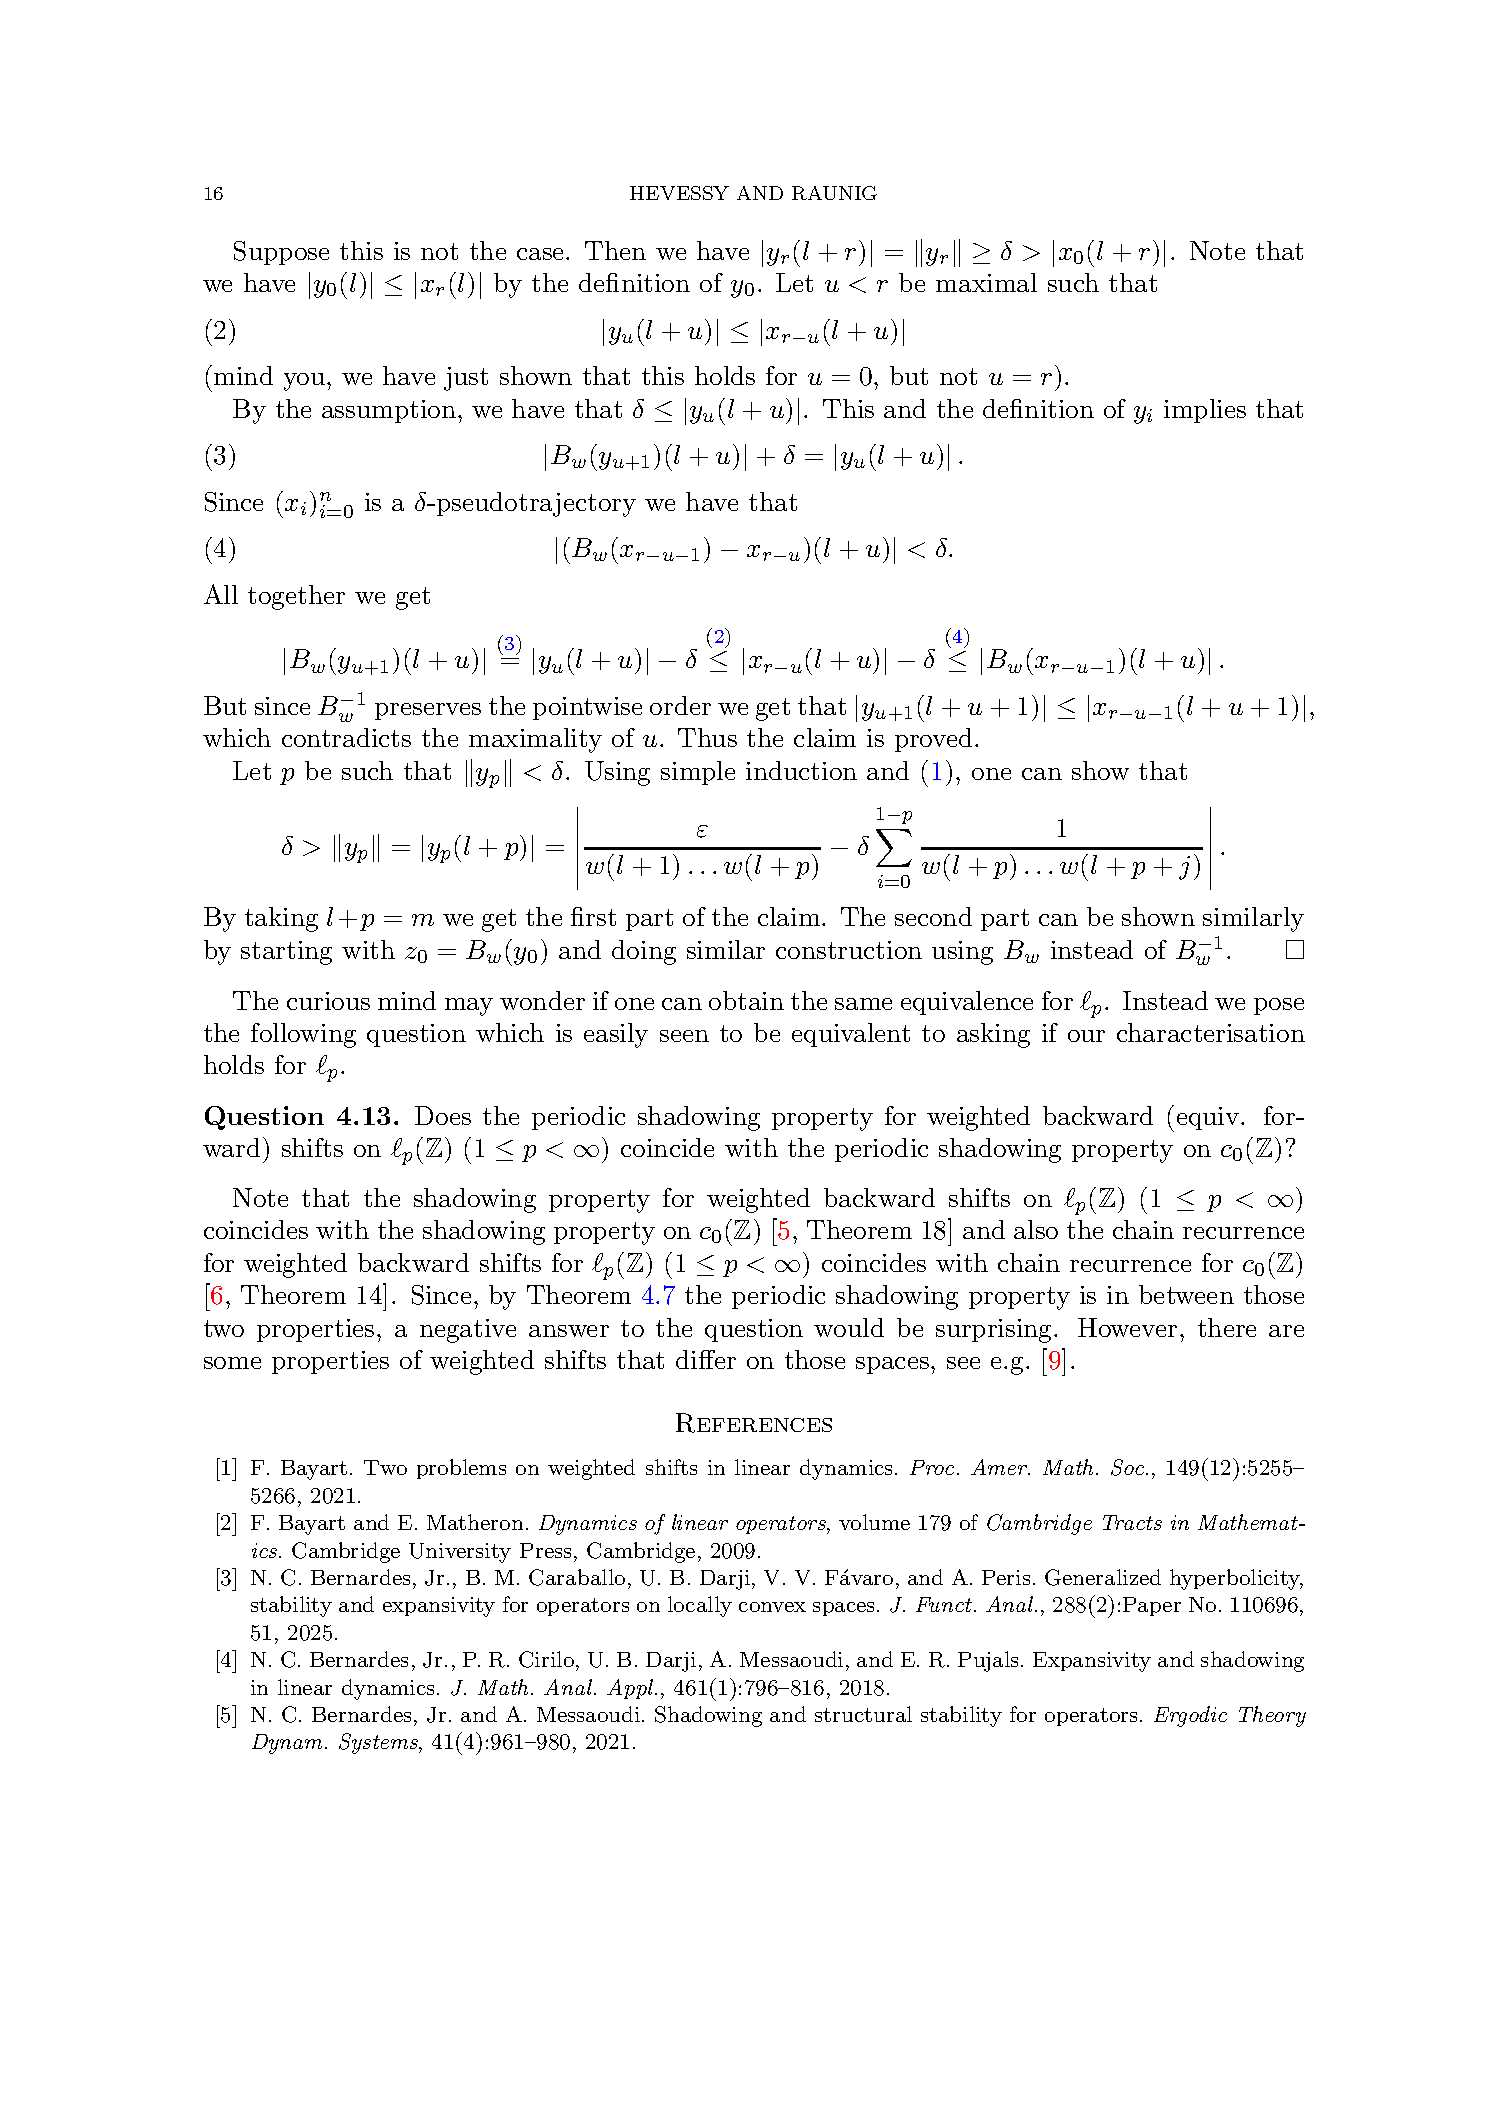
\includegraphics[width=.92\linewidth]{figures/open_question_page16.png}
\end{center}

In the numbering of the rendered arXiv v2 PDF this is Question 4.13: does periodic shadowing for weighted backward, equivalently forward, shifts on \(\ell_p(\Z)\), \(1\leq p<\infty\), coincide with periodic shadowing on \(c_0(\Z)\)?

\section{Proof Intuition}

The only obstruction in the source paper is the case in which the shift has no nonzero periodic points.  In that case, periodic shadowing means that every sufficiently accurate periodic pseudo-orbit must be small, since the only periodic point available to shadow it is \(0\).

For a period \(N\) pseudo-orbit \(x=(x_0,\ldots,x_{N-1})\), write its cyclic defect as
\[
 (D_Nx)_i=x_{i+1}-B_wx_i,\qquad i\in \Z/N\Z .
\]
Thus periodic shadowing with no nonzero periodic points is the uniform estimate
\[
 \max_i\norm{x_i}\leq C\max_i\norm{x_{i+1}-B_wx_i}
\]
for all periods \(N\).

For \(c_0\), this estimate is scalar: the operator \(D_N\) decomposes along the diagonal orbits of the space-time lattice \((i,j)\mapsto(i+1,j-1)\).  The \(c_0\) estimate is exactly a uniform bound on the scalar Green matrices for these first-order diagonal recurrences.  Those matrices have bounded row sums; applying the same argument to the inverse shift gives the corresponding column control.  The Schur test then lifts the scalar estimate to the mixed norm \(\max_i\norm{x_i}_{p}\).  This removes the only missing implication in the source paper.

\section{Preliminaries}

We use three facts from the source paper \cite{HR2025}.

\begin{enumerate}
\item The periodic points of \(B_w\) are either trivial or dense on each of the spaces under consideration; if they are dense, then periodic shadowing is equivalent to the ordinary shadowing property \cite[Proposition 4.5]{HR2025}.
\item The ordinary shadowing property for these weighted shifts is the same on \(\ell_p(\Z)\), \(1\leq p<\infty\), and on \(c_0(\Z)\); the source cites this as Bernardes--Messaoudi's Theorem 18 \cite{BM2021}.
\item If \(\Per(B_w)=\{0\}\), periodic shadowing is equivalent to the following homogeneous cyclic estimate: for every period \(N\) there is one constant \(C\), independent of \(N\), such that every \(N\)-periodic pseudo-orbit satisfies
\[
 \max_{0\leq i<N}\norm{x_i}\leq C
 \max_{0\leq i<N}\norm{x_{i+1}-B_wx_i}.
\]
This is Proposition 4.8 of the source paper, with the usual scaling argument.
\end{enumerate}

We record the only new ingredient separately.

\begin{lemma}[Regular Green-matrix transference]\label{l:transfer}
Assume that \(B_w\) has no nonzero periodic points on \(c_0(\Z)\).  If the cyclic defect estimate above holds on \(c_0(\Z)\), then it holds on \(\ell_p(\Z)\) for every \(1\leq p<\infty\).
\end{lemma}

\begin{proof}
Fix a period \(N\).  For \(x=(x_i)_{i\in\Z/N\Z}\), put \(e=D_Nx\), so
\[
 e_i(j)=x_{i+1}(j)-w_{j+1}x_i(j+1).
\]
For each residue \(r\in\Z/N\Z\), follow the diagonal \(i+j=r\) and define
\[
 a^{(r)}_j=x_{r-j}(j),\qquad b^{(r)}_j=e_{r-j-1}(j),
\]
with time indices understood modulo \(N\).  Then
\[
 a^{(r)}_j-w_{j+1}a^{(r)}_{j+1}=b^{(r)}_j. \tag{1}
\]
Thus \(D_N\) is a direct sum, after this diagonal reindexing, of scalar first-order difference equations.  The \(c_0\) cyclic estimate says that the solution operator for (1), restricted to \(c_0\)-solutions, is bounded in sup norm by a constant \(C\) independent of \(N\) and \(r\).

Apply this estimate first to \(B_w\), and then to \(B_w^{-1}\).  Periodic shadowing is invariant under inversion: reversing a periodic pseudo-orbit of \(B_w\) gives a periodic pseudo-orbit of \(B_w^{-1}\), with constants changed only by the fixed bounds on \(B_w\) and \(B_w^{-1}\).  Consequently the finite Green matrices \(G_N\) associated with (1) have uniformly bounded regular Schur norm: there is \(M\), independent of \(N\), such that for every finite coordinate truncation of the diagonal equations,
\[
 \sup_{\alpha}\sum_{\beta}\abs{(G_N)_{\alpha\beta}}\leq M,
 \qquad
 \sup_{\beta}\sum_{\alpha:\, t(\alpha)=t_0}\abs{(G_N)_{\alpha\beta}}\leq M
\]
for every output time \(t_0\).  The first bound is the sup-norm estimate for arbitrary choices of defect phases; the second is the same row-sum estimate for the reversed cyclic equation, rewritten as a column estimate for a fixed output time.

Now let \(x_i\in\ell_p(\Z)\) and \(e=D_Nx\).  By density it is enough to prove the estimate for finitely supported arrays and then pass to the limit.  Write the Green representation with nonnegative coefficients \(g_{\alpha\beta}=\abs{(G_N)_{\alpha\beta}}\):
\[
 \abs{x_{t_0}(j)}\leq \sum_{\beta} g_{(t_0,j),\beta}\abs{e_\beta}.
\]
Using Jensen's inequality with the row-sum bound and then the time-resolved column bound,
\[
\begin{aligned}
 \norm{x_{t_0}}_p^p
 &\leq M^{p-1}\sum_j\sum_{\beta}g_{(t_0,j),\beta}\abs{e_\beta}^p\\
 &\leq M^p \max_{0\leq i<N}\norm{e_i}_p^p .
\end{aligned}
\]
Taking \(p\)-th roots and then the supremum over \(t_0\) gives
\[
 \max_i\norm{x_i}_p\leq M\max_i\norm{(D_Nx)_i}_p,
\]
with \(M\) independent of \(N\).  This is exactly the cyclic defect estimate on \(\ell_p(\Z)\).
\end{proof}

\section{Main Result}

\begin{theorem}\label{t:main}
Let \(w=(w_n)_{n\in\Z}\) be bounded and satisfy \(\inf_n\abs{w_n}>0\).  Let \(B_w\) be the bilateral weighted backward shift on \(c_0(\Z)\) and on \(\ell_p(\Z)\), \(1\leq p<\infty\).  Then
\begin{align*}
&B_w \text{ has the periodic shadowing property on } c_0(\Z)\\
&\qquad\iff
B_w \text{ has the periodic shadowing property on } \ell_p(\Z).
\end{align*}
\end{theorem}

\begin{proof}
First suppose that \(B_w\) has the periodic shadowing property on \(c_0(\Z)\).

If \(B_w\) has a nonzero periodic point on \(c_0(\Z)\), then the periodic points are dense and the source paper gives periodic shadowing \(\Leftrightarrow\) ordinary shadowing.  Since ordinary shadowing is the same on \(c_0(\Z)\) and \(\ell_p(\Z)\), \(B_w\) has shadowing, hence periodic shadowing, on \(\ell_p(\Z)\).

If \(B_w\) has no nonzero periodic point on \(c_0(\Z)\), then it also has no nonzero periodic point on \(\ell_p(\Z)\), because \(\ell_p(\Z)\subset c_0(\Z)\).  Proposition 4.8 of the source paper converts \(c_0\)-periodic shadowing into the uniform cyclic defect estimate on \(c_0\).  Lemma \ref{l:transfer} transfers that estimate to \(\ell_p\).  Applying Proposition 4.8 again gives periodic shadowing on \(\ell_p(\Z)\).

Conversely suppose that \(B_w\) has periodic shadowing on \(\ell_p(\Z)\).

If \(\Per(B_w)\) is nontrivial on \(\ell_p(\Z)\), then it is dense, and the same argument as above gives ordinary shadowing on \(\ell_p(\Z)\), hence ordinary shadowing and periodic shadowing on \(c_0(\Z)\).

It remains to consider the case \(\Per(B_w)=\{0\}\) on \(\ell_p(\Z)\).  The source paper proves that, in this case, periodic shadowing on \(\ell_p(\Z)\) implies the scalar weight condition appearing in its Theorem 4.12.  If \(c_0(\Z)\) had a nonzero periodic point, then \(c_0\)-chain recurrence would be nontrivial; but chain recurrence for these shifts is the same on \(\ell_p(\Z)\) and \(c_0(\Z)\) by Bernardes--Peris \cite[Theorem 14]{BP2024}, as recalled in the source paper after Question 4.13.  This would contradict the source observation that periodic shadowing with no nonzero periodic points forces the chain recurrent set to be \(\{0\}\).  Thus \(\Per(B_w)=\{0\}\) on \(c_0(\Z)\).  The complete \(c_0\)-characterization in Theorem 4.12 of the source paper now converts the same scalar weight condition into periodic shadowing on \(c_0(\Z)\).
\end{proof}

\begin{corollary}
The same equivalence holds for bilateral weighted forward shifts.
\end{corollary}

\begin{proof}
If \(F_w\) is invertible, then \(F_w^{-1}\) is a weighted backward shift with reciprocal shifted weights.  Periodic shadowing is invariant under inversion, so Theorem \ref{t:main} applies to \(F_w^{-1}\) and hence to \(F_w\).
\end{proof}

\section{Verification and Novelty Notes}

The proof uses the source paper's results for the dense-periodic-points case, the source paper's reduction of the zero-periodic-points case to cyclic pseudo-orbit estimates, and the new regular Green-matrix transference lemma above.

The verifier script in the packet's \texttt{code/} folder checks the finite cyclic model behind Lemma \ref{l:transfer}: after diagonal reindexing, the cyclic defect operator splits into first-order scalar blocks, and the sampled mixed \(\ell_p\) amplification is bounded by the Schur constant computed from the finite Green matrix.  This is only a sanity check of the finite algebra; the proof of Lemma \ref{l:transfer} is the mathematical argument.

Local run indexes were searched for arXiv:2509.11852, the paper title, ``periodic shadowing'', ``weighted backward shifts'', ``ell\_p'', and ``c\_0''.  No duplicate settlement was found.  Web searches for the exact question and close variants found the source arXiv page, a seminar announcement, a ResearchGate mirror, and summary/review pages, but no later paper answering Question 4.13.

Human review should focus on Lemma \ref{l:transfer}, specifically the derivation of the time-resolved column bound from the reversed cyclic equation.

\begin{thebibliography}{9}

\bibitem{HR2025}
M. Hevessy and T. Raunig,
\emph{Dynamical properties of weighted shifts on sequence spaces},
arXiv:2509.11852v2, 2025.

\bibitem{BM2021}
N. C. Bernardes Jr. and A. Messaoudi,
\emph{Shadowing and structural stability for operators},
Ergodic Theory Dynam. Systems 41 (2021), no. 4, 961--980.

\bibitem{BP2024}
N. C. Bernardes Jr. and A. Peris,
\emph{On shadowing and chain recurrence in linear dynamics},
Adv. Math. 441 (2024), Paper No. 109539.

\end{thebibliography}

\end{document}
